\section{Using Multipliers (Zone and/or Window)}\label{using-multipliers-zone-andor-window}

\subsection{Background and Study using Multipliers}\label{background-and-study-using-multipliers}

Multipliers are used in EnergyPlus for convenience in modeling. Though window multipliers are useful for any size building when you have multiple windows on a façade, zone multipliers are more useful in large buildings with several to many stories.

Zone multipliers are designed as a ``multiplier'' for floor area, zone loads, and energy consumed by internal gains. It takes the calculated load for the zone and multiplies it, sending the multiplied load to the attached HVAC system. The HVAC system size is specified to meet the entire multiplied zone load and will report the amount of the load met in the Zone/Sys Sensible Heating or Cooling Energy/Rate report variable. Autosizing automatically accounts for multipliers. Metered energy consumption by internal gains objects such as Lights or Electric Equipment will be multiplied.

To illustrate the benefits (and comparison of results), the MultiStory.idf example file was used. The MultiStory file is a 9 zone, 10 story/floored building with heating (ZoneHVAC:Baseboard:Convective:Electric object) and cooling (ZoneHVAC:WindowAirConditioner object). The middle zone of each floor in the original represents 4 zones (multiplier = 4) and the middle floor (ZoneGroup) represents 8 floors (ZoneGroup multiplier = 8). Clone representations were made for comparisons:

\begin{figure}[hbtp] % fig 7
\centering
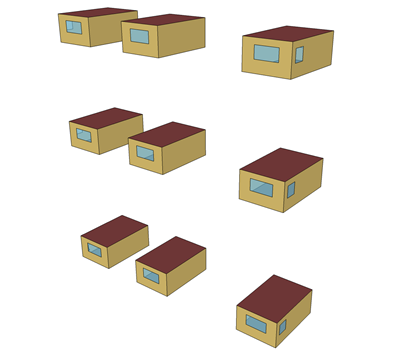
\includegraphics[width=0.9\textwidth, height=0.9\textheight, keepaspectratio=true]{media/image007.png}
\caption{Original Multistory IDF \protect \label{fig:original-multistory-idf}}
\end{figure}

In the figure above, each ``middle'' zone represents 4 zones.~ The middle ``floor'' represents 8 floors. Additionally, each of the windows has a multiplier of 4 -- so each window represents 4 windows of the same size. For the Multistory file, the Zone object for the center zones has the multiplier of 4. And for the center floors, the ZoneList and ZoneGroup objects to collect the zones and apply multipliers. The top floor then uses the Zone object multiplier for the center zones. Specifically:

\begin{lstlisting}

<snip>
    Zone,
      Gnd Center Zone,         !- Name
      0.0,                     !- Direction of Relative North {deg}
      8.0, 0.0, 0.0,           !- Origin [X,Y,Z] {m}
      1,                       !- Type
      4,                       !- Multiplier
      autocalculate,           !- Ceiling Height {m}
      autocalculate;           !- Volume {m3}
  <snip>

    ZoneGroup,
      Mid Floor,               !- Zone Group Name
      Mid Floor List,          !- Zone List Name
      8;                       !- Zone List Multiplier


    ZoneList,
      Mid Floor List,          !- Zone List Name
      Mid West Zone,           !- Zone 1 Name
      Mid Center Zone,         !- Zone 2 Name
      Mid East Zone;           !- Zone 3 Name
  <snip>

    Zone,
      Top Center Zone,         !- Name
      0.0,                     !- Direction of Relative North {deg}
      8.0,                     !- X Origin {m}
      0.0,                     !- Y Origin {m}
      22.5,                    !- Z Origin {m}
      1,                       !- Type
      4,                       !- Multiplier
      autocalculate,           !- Ceiling Height {m}
      autocalculate;           !- Volume {m3}
\end{lstlisting}

For comparison purposes, clones of the middle zones were done.

\begin{figure}[hbtp] % fig 8
\centering
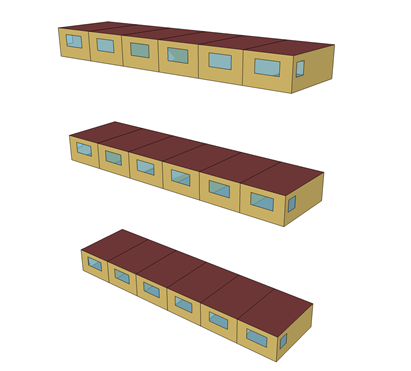
\includegraphics[width=0.9\textwidth, height=0.9\textheight, keepaspectratio=true]{media/image008.png}
\caption{Multistory with cloned middle zones. \protect \label{fig:multistory-with-cloned-middle-zones.}}
\end{figure}

And, finally, the entire building was created:

\begin{figure}[hbtp] % fig 9
\centering
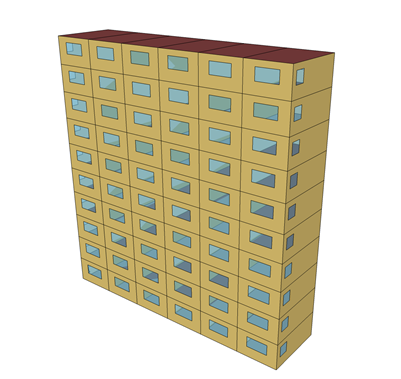
\includegraphics[width=0.9\textwidth, height=0.9\textheight, keepaspectratio=true]{media/image009.png}
\caption{Multistory building -- fully cloned. \protect \label{fig:multistory-building-fully-cloned.}}
\end{figure}

The building is autosized. For convenience in comparison, the extreme summer and winter days were used for autosizing and the simulation was run for the 5 United States weather files that are included in the EnergyPlus release: Chicago IL; San Francisco CA; Golden CO; Tampa FL; and Washington DC.

Comparisons were done with the Zone Group Loads values (Zone Group Sensible Heating Energy and Zone Group Sensible Cooling Energy) as well as meter values for Electricity. Using the regression testing limits that are used during EnergyPlus development testing (i.e.~small differences are within .001 or .5\%; big differences are greater than those limits).

For the purposes of dicussion, the buildings will be called: Multistory 1 -- the original 9 zone building (with multipliers and groups) ref: Figure~\ref{fig:original-multistory-idf}; Multistory 2 -- the building shown in Figure~\ref{fig:multistory-with-cloned-middle-zones.}. Multistory with cloned middle zones.; Multistory 3 -- the fully configured building -- ref Figure~\ref{fig:multistory-building-fully-cloned.}.

The following table illustrates the regression testing for Multistory 2 and Multistory 3, group loads and meters versus Multistory 1 results.  For these tables, the location indicators refer to the following EnergyPlus weather files: Chicago (USA IL Chicago-OHare.Intl.AP.725300 TMY3), San Francisco (USA CA San.Francisco.Intl.AP.724940 TMY3), Colorado(USA CO Golden-NREL.724666 TMY3), Tampa (USA FL Tampa.Intl.AP.722110 TMY3), and Washington DC(USA VA Sterling-Washington.Dulles.Intl.AP.724030 TMY3).

% table 1
\begin{longtable}[c]{p{1.2in}p{1.2in}p{1.2in}p{1.2in}p{1.2in}}
\caption{Multistory vs Multistory 2 and Multistory 3 \label{table:multistory-vs-multistory-2-and-multistory-3}} \tabularnewline
\toprule 
LOCATION & MULTI-STORY 2 LOADS & MULTI-STORY 2 METER & MULTI-STORY 3 LOADS & MULTI-STORY 3 METER \tabularnewline
\midrule
\endfirsthead

\caption[]{Multistory vs Multistory 2 and Multistory 3} \tabularnewline
\toprule 
LOCATION & MULTI-STORY 2 LOADS & MULTI-STORY 2 METER & MULTI-STORY 3 LOADS & MULTI-STORY 3 METER \tabularnewline
\midrule
\endhead

Chicago & Small Diffs & Equal & Big Diffs* (76\%) & Big Diffs* (62\%) \tabularnewline
San Francisco & Big Diffs* (2.43\%) & Big Diffs* (0.6\%) & Big Diffs* (49\%) & Big Diffs* (41\%) \tabularnewline
Colorado & Small Diffs & Small Diffs & Big Diffs* (26\%) & Big Diffs* (24\%) \tabularnewline
Tampa & Small Diffs & Small Diffs & Big Diffs* (6\%) & Big Diffs* (2\%) \tabularnewline
Washington DC & Equal & Equal & Big Diffs* (91\%) & Big Diffs* (72\%) \tabularnewline
\bottomrule
\end{longtable}

* Big Diffs maximum occur in monthly values whereas the runperiod values are much smaller.

To try to pare down the discrepancies shown here, the effects of height that are used in the calculations were removed (i.e., the Site:WeatherStation and Site:HeightVariation objects were entered as below to negate the effects of height on the environmental variables such as wind and temperature).~ In addition the height effect was removed from the OutdoorAir:Node object.

\begin{lstlisting}

  Site:WeatherStation,
      ,          !- Wind Sensor Height Above Ground {m}
      ,          !- Wind Speed Profile Exponent
      ,          !- Wind Speed Profile Boundary Layer Thickness {m}
      0;         !- Air Temperature Sensor Height Above Ground {m}


    Site:HeightVariation,
      0,         !- Wind Speed Profile Exponent
      ,          !- Wind Speed Profile Boundary Layer Thickness {m}
      0;         !- Air Temperature Gradient Coefficient {K/m}
\end{lstlisting}

Figure 10. Objects removing height from building impacts.

With these included, the files were rerun with the following results:

% table 2
\begin{longtable}[c]{p{1.2in}p{1.2in}p{1.2in}p{1.2in}p{1.2in}}
\caption{Multiplier Results with negated height variation. \label{table:multiplier-results-with-negated-height}} \tabularnewline
\toprule 
Location & Multi-story 2 Loahs & Multi-story 2 Meter & Multi-story 3 Loahs & Multi-story 3 Meter \tabularnewline
\midrule
\endfirsthead

\caption[]{Multiplier Results with negated height variation.} \tabularnewline
\toprule 
Location & Multi-story 2 Loahs & Multi-story 2 Meter & Multi-story 3 Loahs & Multi-story 3 Meter \tabularnewline
\midrule
\endhead

Chicago & Small diffs & Small diffs & Small diffs & Small diffs \tabularnewline
San Francisco & Small diffs & Small diffs & Small diffs & Small diffs \tabularnewline
Colorado & Small diffs & Small diffs & Small diffs & Small diffs \tabularnewline
Tampa & Small diffs & Small diffs & Small diffs & Small diffs \tabularnewline
Washington DC & Small diffs & Small diffs & Small diffs & Small diffs \tabularnewline
\bottomrule
\end{longtable}

To investigate if other systems might have different results, the Ideal Loads System was used as the system.~ Similar results were found for the multipliers vs cloned results. However, it may also be noted that the results between the original systems (baseboard and window ac) vs the ideal loads were very similar.

The biggest difference really comes in calculation time. As shown in the following table,

% table 3
\begin{longtable}[c]{p{1.5in}p{1.5in}p{1.5in}p{1.5in}}
\caption{Runtimes for Multistory files (baseboard/window ac) \label{table:runtimes-for-multistory-files-baseboardwindow}} \tabularnewline
\toprule 
Location & Multi-story 1 (9 zones) (mm:ss) & Multi-story 2~ (18 zones) (MM:SS) & Multi-story 3 (60 zones) (MM:SS) \tabularnewline
\midrule
\endfirsthead

\caption[]{Runtimes for Multistory files (baseboard/window ac)} \tabularnewline
\toprule 
Location & Multi-story 1 (9 zones) (mm:ss) & Multi-story 2~ (18 zones) (MM:SS) & Multi-story 3 (60 zones) (MM:SS) \tabularnewline
\midrule
\endhead

Chicago & 1:05 & 2:14 & 13:15 \tabularnewline
San Francisco & 1:04 & 2:05 & 13:20 \tabularnewline
Colorado & 1:17 & 2:28 & 14:43 \tabularnewline
Tampa & 1:11 & 2:21 & 13:43 \tabularnewline
Washington DC & 1:05 & 2:15 & 13:18 \tabularnewline
\bottomrule
\end{longtable}

Because the overall results were so similar, the run times for the Ideal Loads runs are included:

% table 4
\begin{longtable}[c]{p{1.5in}p{1.5in}p{1.5in}p{1.5in}}
\caption{Runtime for Multistory files (ideal loads) \label{table:runtime-for-multistory-files-ideal-loads}} \tabularnewline
\toprule 
Location & Multi-story 1 (9 zones) (mm:ss) & Multi-story 2 (18 zones) (MM:SS) & Multi-story 3 (60 zones) (MM:SS) \tabularnewline
\midrule
\endfirsthead

\caption[]{Runtime for Multistory files (ideal loads)} \tabularnewline
\toprule 
Location & Multi-story 1 (9 zones) (mm:ss) & Multi-story 2 (18 zones) (MM:SS) & Multi-story 3 (60 zones) (MM:SS) \tabularnewline
\midrule
\endhead

Chicago & 0:51 & 1:34 & 9:37 \tabularnewline
San Francisco & 0:50 & 1:34 & 9:59 \tabularnewline
Colorado & 0:51 & 1:40 & 10:31 \tabularnewline
Tampa & 0:51 & 1:36 & 10:05 \tabularnewline
Washington DC & 0:51 & 1:36 & 9:48 \tabularnewline
\bottomrule
\end{longtable}

More zones (and, particularly more surfaces) make for longer run times.

\subsection{Guidelines for Using Multipliers and Groups}\label{guidelines-for-using-multipliers-and-groups}

\begin{itemize}
\item
  If the basic zone geometry is identical, make one zone, copy \& paste it as necessary, then change the Zone Origin field to locate each zone correctly.
\item
  Do not use interzone surfaces between zones that are multiplied. Set the adjoining surfaces to be adiabatic, i.e.~use the OtherZoneSurface exterior boundary condition with the other surface pointing back to itself.
\item
  Locate the middle floor zones roughly halfway between top and ground because exterior convection coefficients change with height. Halfway should cause the differences to average out. If you have many stories (the example only has 10 stories), consider using more middle floor zones.
\item
  Consider removing the effects of height variation for the simulation.
\item
  Follow guidelines in HVACTemplate and other objects about sizing if you are mixing autosize fields with hard sized fields (recommended to ``autosize'' all fields rather than mix).
\item
  All HVAC system sizes must be specified to meet the entire multiplied zone load.
\item
  Autosizing automatically accounts for multipliers.
\end{itemize}
